\chapter{Large Deviation}

\begin{center}
\textbf{\large verbatim from Leighton F08.lecture25-devs}
\end{center}

\section{Chernoff Bounds}
The bounds we get using the Markov Theorem and the Chebyshev Theorem are
sometimes very good, and sometimes very bad. Now we're going to turn to a
special case of a random variable which arises in practice. The special
case is when the random variable is the sum of lots of other random
variables that are mutually independent, and the bound on the probability
of deviating from the mean is known as the Chernoff bound. Chernoff was a
professor here, and at the time of discovery did not put much importance
on his bounds, which were much later applied by many others in many
situations.

\iffalse
MIT is admitting a new crop of students.  The Institvte has offered
admission to a few thousand applicants and carefully estimated the
probability that each will accept, based on his or her interests,
enthusiasm, and other likely offers.  This calculation indicates that
the expected number of new students is 1000, which is the ideal
number.  However, MIT must be wary of weird happenings.  If the new
class is too small, then expenses must be divided among fewer
students, forcing tuition up.  If the new class is too large, then
living conditions and classes will be crowded.  What is the
probability that MIT must cope with significantly fewer or more
students?

Similar problems arise again and again in the analysis of computer
systems and algorithms.  The general theme is that there are many
events that \textit{can} occur, and we need to prove that the number
that actually \textit{do} occur is unlikely to be much greater or much
less than the expected number.  In terms of the probability density
function, we're trying to show that the tails are small:
%
\begin{center}
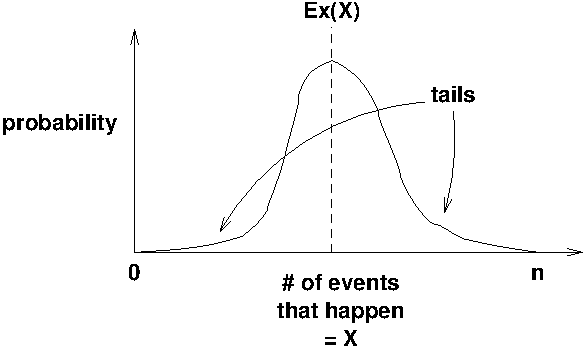
\includegraphics{pdf-x2}
\end{center}
%
If the events are mutually independent, then we can get quick results
to this effect from a powerful set of tools called \term{Chernoff
bounds}.
\fi

\begin{theorem}[Chernoff Bounds]
\label{th:chernoff}
Let $T_1, \ldots, T_n$ be any mutually independent random variables such that $\forall j$, $0 \leq T_j \leq 1$. Let 
$T = \sum_{j=1}^N T_j$. Then for any $c > 1$, 
$$\pr{T \geq c \expect{T}} \leq e^{-\alpha \expect{T}},$$
where $\alpha = c\ln c + 1 - c > 0$.
\end{theorem}
In general this is a much better bound than you get from Markov or Chebyshev. 
The probability from Markov is $1/c$. The bound from Chebyshev is only 
slightly better. With Chernoff, the bound is exponentially small in $c\ln c$ 
times the expected value. This is a huge difference. 

For example, using Chernoff Bounds, $\pr{T \geq 2 \expect{T}} \leq
e^{-38}$ if $\expect{T} = 100$. In this case Markov would only give $1/2$,
and the one-sided extension of Chebyshev would only give $1/(10^2 +1) =
1/101$, which we can show by bounding $\expect{T}$ with $\variance{T}$:

\begin{align}
\pr{T\geq 2\cdot\expect{T}}
& = \pr{T-\expect{T}\geq \expect{T}}\\
& = \pr{T-\expect{T}\geq c\cdot\sigma(T)}\\
& \leq\frac{1}{c^2+1}\\
& \leq\frac{1}{\expect{T}+1}\\
& =\frac{1}{101}\\
\end{align}

In line 1, we subtract $\expect{T}$ from both sides of the
inequality. In line 2, we make the substitution $\expect{T}=c\cdot
\sigma(T)$. We use the one-sided Chebyshev bound in the third line. In
step 4, we make use of the fact that for the random variable $T$, we
know $\sigma^2(T)\leq\expect{T}$, a result which we derived during
recitation yesterday. This fact tells us that
$\sigma(T)\leq\sqrt{\expect{T}}$, which we can use to bound $c$: $c =
\frac{\expect{T}}{\sigma(T)} \geq \sqrt{\expect{T}}$. In the final
step, we use the fact that in this example, $\expect{T}=100$. This
result is decent (certainly better than the bounds derived from the
Markov Theorem!), but the Chernoff result is much better.

Of course, Chernoff Bounds do not apply to all distributions. They only work when $R$ is the sum of random variables defined on the interval $[0,1]$. But this is a pretty broad class, and includes, for example, the binomial distribution. In fact, the $T_j$ form a much broader class since the $T_j$ need not have the same distribution, and their distribution can be arbitrary on the interval $[0,1]$, rather than just Bernoulli. 

Another nice thing about the Chernoff Bound is that the bound does not directly depend on the number of random variables being summed, and you can show that even small deviations are unlikely. 

For example, suppose $10$ million people play ``Pick 4''. This is a lottery game where you pick a $4$-digit number and you win if you get an exact match. Then the probability of winning is just $\pr{\textrm{Win}} = \frac{1}{10000}$, and the expected number of winners is $10$ million divided by ten thousand, or $1000$. 

Suppose each of the $10$ million players pick mutually independent random numbers. Then by Chernoff Bounds, we know $\pr{\geq 2000 \textrm{ winners}} \leq e^{-.38 \cdot 1000} = e^{-380}$. Moreover, $\pr{\geq 1100 \textrm{ winners}} \leq e^{-4.8} < .01$, so only a $1\%$ chance that the number of winners is $10\%$ over the expectation. Note that the Markov and Chebyshev Theorems are useless here. 

So let's prove the theorem. Then we'll apply it to load balancing. The proof of the theorem is similar to the proof of Chebyshev's Theorem. As in the proof of Chebyshev, we'll use Markov's Theorem, but in this case, we exponentiate the deviation instead of squaring it before applying Markov's Theorem. The proof is clever and a bit tricky. We don't expect you to be able to derive such a proof on your own in this class.

\begin{proof}
\noindent Define $R_j = T_j - \expect{T_j}$ for $j = 1, 2, \ldots, N$. Then 
$$-\expect{T_j} \leq R_j \leq 1- \expect{T_j},$$
and $\expect{R_j} = 0$. We have,
\begin{eqnarray*}
\pr{T \geq c \expect{T}} & = & \pr{R \geq (c-1)\expect{T}}\\
& = & \pr{c^R \geq c^{(c-1)\expect{T}}}\\
& \leq & \frac{\expect{c^R}}{c^{(c-1)\expect{T}}} \ \ \textrm{ Markov's Bound}.
\end{eqnarray*}
Thus,
\begin{eqnarray*}
\expect{c^R} & = & \expect{c^{R_1 + R_2+ \cdots + R_N}}\\
& = & \expect{\Pi_{j=1}^N c^{R_j}}\\
& = & \Pi_{j=1}^N \expect{c^{R_j}} \ \ \textrm{ independence of the }T_j \textrm{ and thus } R_j.
\end{eqnarray*}
We need the following facts.
\begin{fact}
If $-m \leq z \leq 1-m$, then $c^z \leq c^{-m}(1 + m(c-1)) + z(c^{1-m} - c^{-m})$.
\end{fact}
This follows from the fact that the right-hand-side describes a line which intersects the curve $c^z$ (here $z$ is the variable) at $z = -m$ and $z = 1-m$. Moreover, since $c^z$ is convex, the curve is entirely below this line. 
\begin{fact}
$1 + m(c-1) \leq e^{m(c-1)}$.
\end{fact}
This follows from the Taylor expansion $1 + x \leq e^x$. 
\\\\
Resuming the proof, set $m = \expect{T_j}$ and $z = R_j$. Then
\begin{eqnarray*}
\expect{c^{R_j}} &\leq &\expect{c^{-m}e^{m(c-1)} + (c^{1-m} - c^{-m})R_j}\\
& = & c^{-m}e^{m(c-1)} \ \ \textrm{ since } \expect{R_j} = 0\\
& = & e^{m(c-1-\ln c)}
\end{eqnarray*}
Thus,
\begin{eqnarray*}
\Pi \expect{c^{R_j}} & \leq & \Pi e^{\expect{T_j}(c-1-\ln c)}\\
& = & e^{(c-1-\ln c)\sum \expect{T_j}}\\
& = & e^{(c-1-\ln c)\expect{T}}
\end{eqnarray*}
Concluding,
\begin{eqnarray*}
\pr{T \geq c\expect{T}} & \leq & \frac{e^{(c-1-\ln c)\expect{T}}}{c^{(c-1)\expect{T}}}\\
& = & e^{\expect{T}(c - 1- \ln c - c\ln c + \ln c)}\\
& = & e^{\expect{T}(-c \ln c - 1 + c)}\\
& = & e^{-\alpha \expect{T}},
\end{eqnarray*}
where $\alpha = c\ln c 1-c$.
\end{proof}

%%%%%%%%%%%%%%%%%%%%%%%%%%%%%%%%%%%%%%%%%%%%%%%%%%%%%%%%%%%%%%%%%%%%%%%%%%%%%%%
\section{Load Balancing}
Suppose we need to build a load balancing device to assign a set of $N$ jobs $B_1, B_2, \ldots, B_N$ to a set of $m$ servers $S_1, S_2, \ldots, S_m$. If you are hosting a decent-sized website, $N$ might be about $100K$ and $m$ might be about $10$. Suppose the $i$th job $B_j$ takes $L_j$ time, $0 \leq L_j \leq 1$ (say, in seconds). The goal is to assign the $N$ jobs to the $m$ servers so that the load is as balanced as possible (i.e., so that the busiest server finishes as quickly as possible). 

Suppose each server works sequentially through the jobs that are assigned to it and finishes in time equal to the sum of job lengths assigned to the server. Let $L_{Tot} = \sum_{j=1}^N L_j$ be the total sum of job lengths. With perfect load balancing then, each server would take $L_{Bal} = \frac{L_{Tot}}{m}$ time. Now if you know the $L_j$, this is a variant of the knapsack problem. It is hard to get all the tasks perfectly balanced but good algorithms exist to get close.

But we are interested in the case when you don't know the job lengths until after you make the assignments, which is often the case in practice. At first it seems hopeless. The idea, however, is to assign the jobs randomly, i.e., to pick $1$ of $m$ processors uniformly at random for each job. This is a very useful technique in computer science when you don't have enough information to solve a problem or a deterministic solution is too hard to figure out. 

Let's see how it works in this case. Normally this kind of technique isn't covered until grad school, but we're ready for it now! We'll start by seeing how much load gets assigned to the $i$th server $S_i$. 

Let $R_{i,j}$ be the load on $S_i$ from job $B_j$. Then $R_{i,j} = L_j$ if $B_j$ is assigned to $S_i$, and is $0$ otherwise. Note, $0 \leq R_{i,j} \leq 1$. Let $R_i$ be the total load on $S_i$ from all jobs. Then $R_i = \sum_{j=1}^N R_{i,j}$. So,
\begin{eqnarray*}
\expect{R_i} & = & \sum_{j=1}^N \expect{R_{i,j}} \\
& = & \sum_{j=1}^N L_j/m\\
& =& \frac{1}{m} L_{Tot}\\
& = & L_{Bal}.
\end{eqnarray*}
So the expected load on the $i$th server is what we would get if the load were perfectly balanced. Because of mutual independence and that $0 \leq R_{i,j} \leq 1$, we can apply Chernoff's Bound. Thus, $\pr{R_i \geq cL_{Bal}} \leq e^{-\alpha L_{Bal}}$, where $\alpha = c\ln c + 1-c$. 

Now this holds for each $i$ individually, but we need to make sure that none of the servers has too much load. To do this, we need to bound the probability that the worst server takes more than $cL_{Bal}$ steps. This is just
$$\pr{R_1 \geq cL_{Bal} \vee R_2 \geq cL_{Bal} \vee \cdots \vee R_m \geq cL_{Bal}}.$$
We can upper bound this by summing the probabilities,
$$\leq \pr{R_1 \geq cL_{Bal}} + \cdots + \pr{R_m \geq cL_{Bal}} \leq me^{-\alpha L_{Bal}}.$$
For example, if we plug in $c = 1.1$ ($10\%$ above the optimal), $\alpha  > .0048$. Let $N = 100K$ and $m = 10$. Say the average job is $1/4$ seconds. Then $L_{Tot} = 25K$, and $L_{Bal} = 2500$. Then, $\pr{\exists \textrm{ server with } \geq 10\% \textrm{ extra load }} \leq 10 e^{-.0048 \cdot 2500} < e^{-9}$.

Thus, our randomized algorithm got all $10$ servers to within $10\%$ of the optimal load with very high probability. This gives a very nice performance, especially compared to the worst case. The only way we do poorly is if we have a bad random assignment; that is, this result holds no matter what the job lengths are. This is a really useful and powerful tool in computer science.
\end{document}
